\chapter{Project Design}

This chapter outlines the design behind each component of the NLP model and the respected process each component may entail, several components will execute more than one step to achieve the desired result. The design is reflected within the final model and each component is broken down to display the functionality and theory within this project. Within section \ref{section:FunctionalRequirements}, it is detailed there won’t be a GUI for the interaction and thus the design section relates to the inner workings of the model itself, that being: system architecture, logistics and theory.

\section{Classical vs Modern}

As originally intended, this project would have seen two differing implementations of the same concept, one being of a classical nature and the other being a machine learning variation, as previously mentioned this project experienced time management issues due to unexpected issue, to which resulted in only focusing on the machine learning implementation of a novel approach. The design for the first model would have been of the following:

\begin{figure}[H]
    \centering
    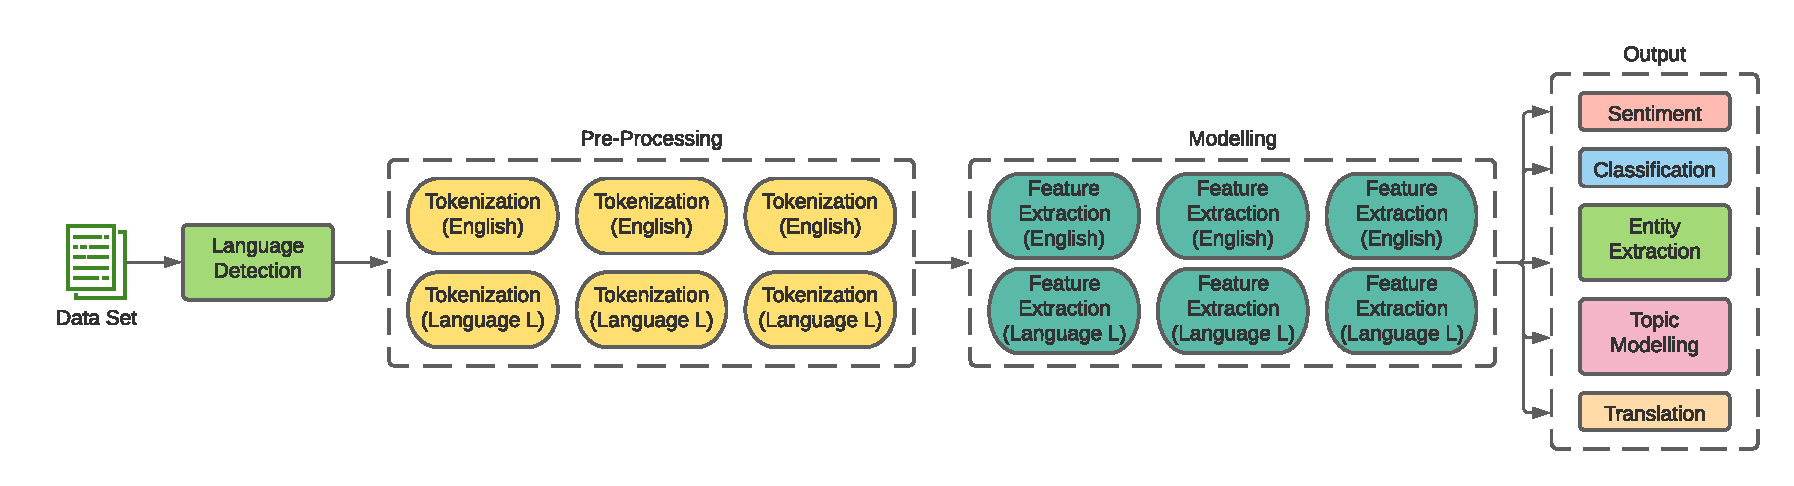
\includegraphics[width=\textwidth]{figures/chapter-5/ClassicalNLP.pdf}
    \caption[ClassicalNLP]{Classical NLP pipeline for text classification.
    \label{fig:ClassicalNLP}}
\end{figure}

Classical or traditional methods for NLP include: (Continuous)Bag-Of-Words, N-Gram, Hidden Markov Models using Markov Chains and Part-Of-Speech Tagging. The developer had originally intended to implement a traditional approach within a machine learning model. The combination of Bag-Of-Words with a machine learning model to calculate a word’s vector based on its TF-IDF value would have been the start, such that:

\begin{equation}
    tf(t,d) = \frac{f_t, _d}{\sum{t \in_d} f _t {_`}, _d}
\end{equation}

It would have also used the inverse TF-IDF value as the project model covers multiple datasets, such that:

\begin{equation}
    idf(t, D) = \log \frac{N}{|d \in D : t \in d|}
\end{equation}

Where the traditional aspect of the Bag-of-Words would produce a vector for each item in a corpus, it’s TF-IDF value would have been calculate through a series of CNN nodes.

Machine learning concepts can be classed as a “black-box” of functionality as the user does not necessarily see what is being executed within the hidden layers, a high-level abstraction for this project can be generalised into the following diagram:

\begin{figure}[H]
    \centering
    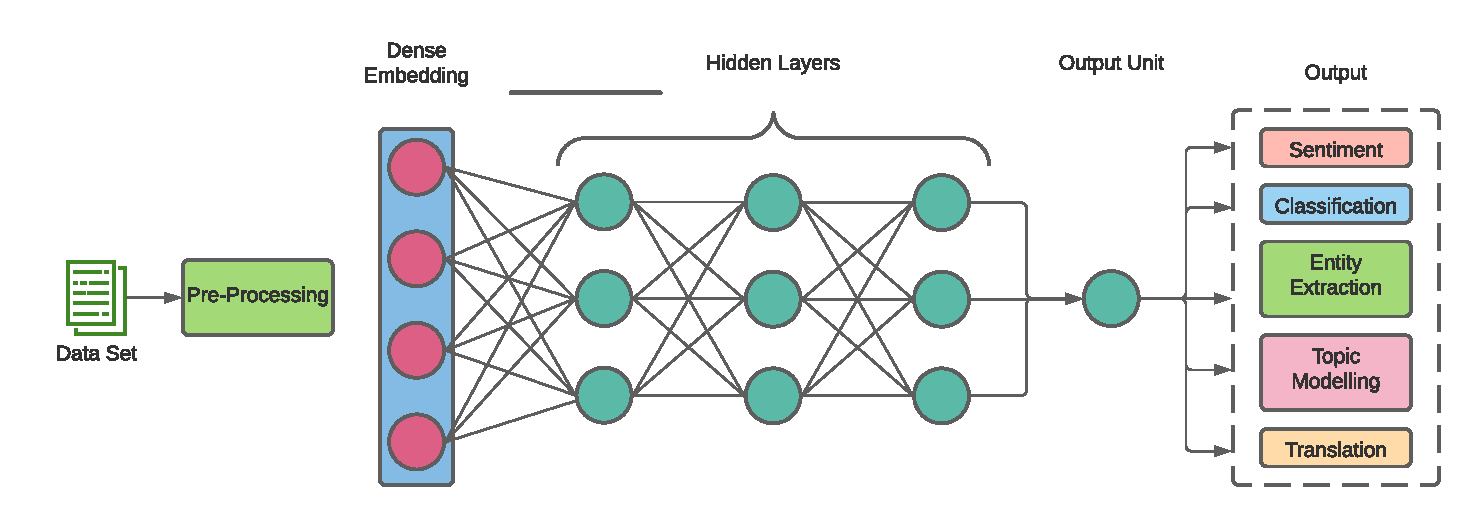
\includegraphics[width=\textwidth]{figures/chapter-5/MLNLP.pdf}
    \caption[MachineLearningNLP]{Machine Learning Model for an NLP pipeline for text classification.
    \label{fig:MLNLP}}
\end{figure}

\section{Planning the ML Model Design}

Initial prototyping of the machine learning model for a new amalgamation of NLP techniques helped to indicate what the best route of development could be, the planning stage piggybacked off existing work flowchart diagrams in-order to choose the most appropriate method and technique combination. The sequence flowchart is as follows:

\begin{figure}[H]
    \centering
    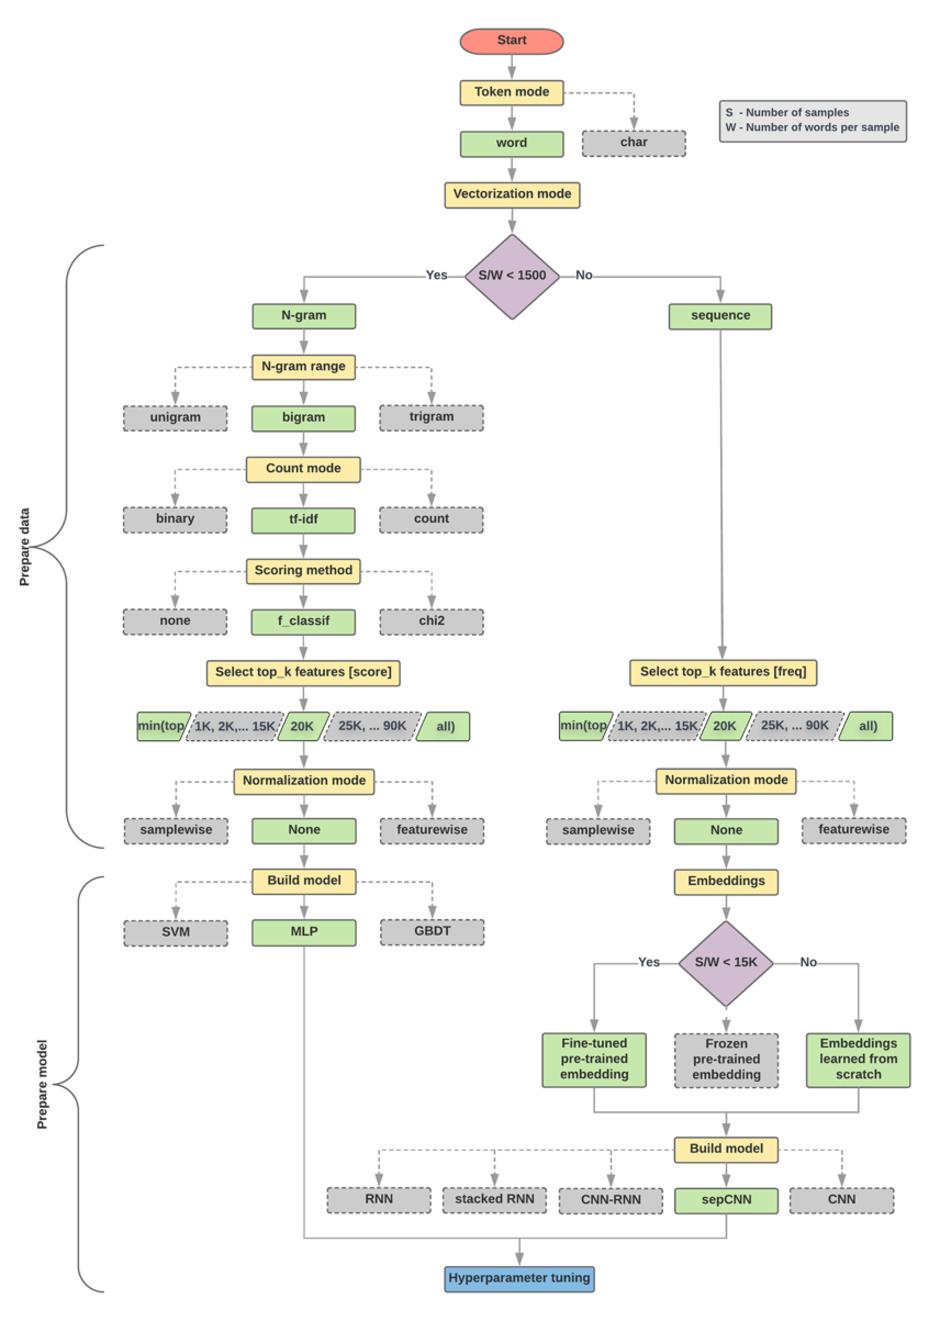
\includegraphics[width=\textwidth]{figures/chapter-5/GooglePlan.pdf}
    \caption[GooglePlan]{Text Classification Flowchart \parencite{google2021TCF}.
    \label{fig:GooglePlan}}
\end{figure}

\section{Supervision}

The development of the project model is based on a supervised approach due to the datasets located, it was most appropriate to use a supervised approach due to the datasets having no labels or lexical categories to train the model on; the model has user input to account for missing labels on data which have been manually and algorithmically added. The supervision for this project can be represented as the following diagram:

\begin{figure}[H]
    \centering
    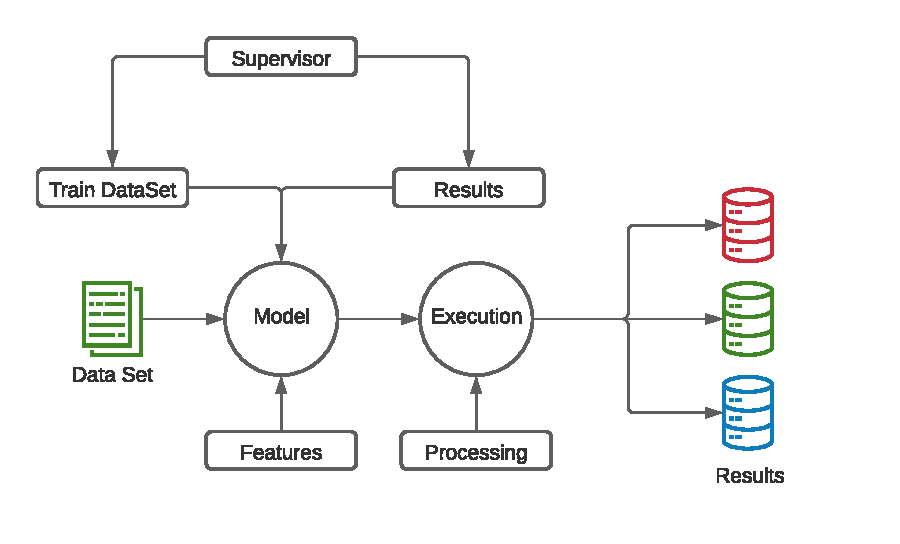
\includegraphics[width=\textwidth]{figures/chapter-5/SupervisedLearningChart.pdf}
    \caption[SupervisedLearning]{Sequence control for Supervised learning.
    \label{fig:SupervisedLearningChart}}
\end{figure}

\section{Pipeline Design}

\begin{figure}[H]
    \centering
    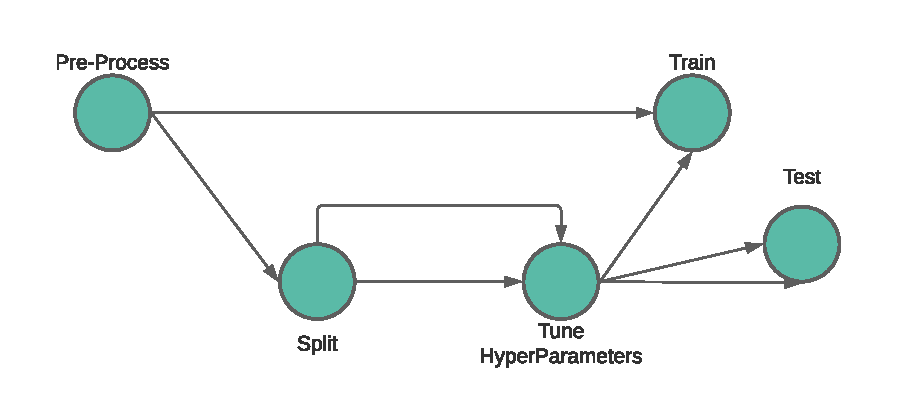
\includegraphics[width=\textwidth]{figures/chapter-5/Pipeline.pdf}
    \caption[MLTCPipeline]{Pipeline for model classification.
    \label{fig:MLTCPipeline}}
\end{figure}

There are five main steps for a text classification pipeline:

\begin{enumerate}
    \item \textbf{\textit{Pre-processing}}: prepare the raw dataset to be trained.
    \item \textbf{\textit{Splitting}}: split the processed dataset to be trained and validated.
    \item \textbf{\textit{Tuning}}: identity valuable parameters within trained data.
    \item \textbf{\textit{Training}}: train the current iteration of the model with updated hyper-parameters.
    \item \textbf{\textit{Testing}}: test and collect statistics for analysis to make further predictions.
\end{enumerate}

\section{Data Preparing and Pre---processing}

Data Preparing

\section{Model}

Skip-gram rather than CBOW as it yields better results with large datasets - such as student feedback - skip gram can also be context aware as it converts neighboring lexemes to vectors

\subsection{Skip-Gram}

\begin{figure}[H]
    \centering
    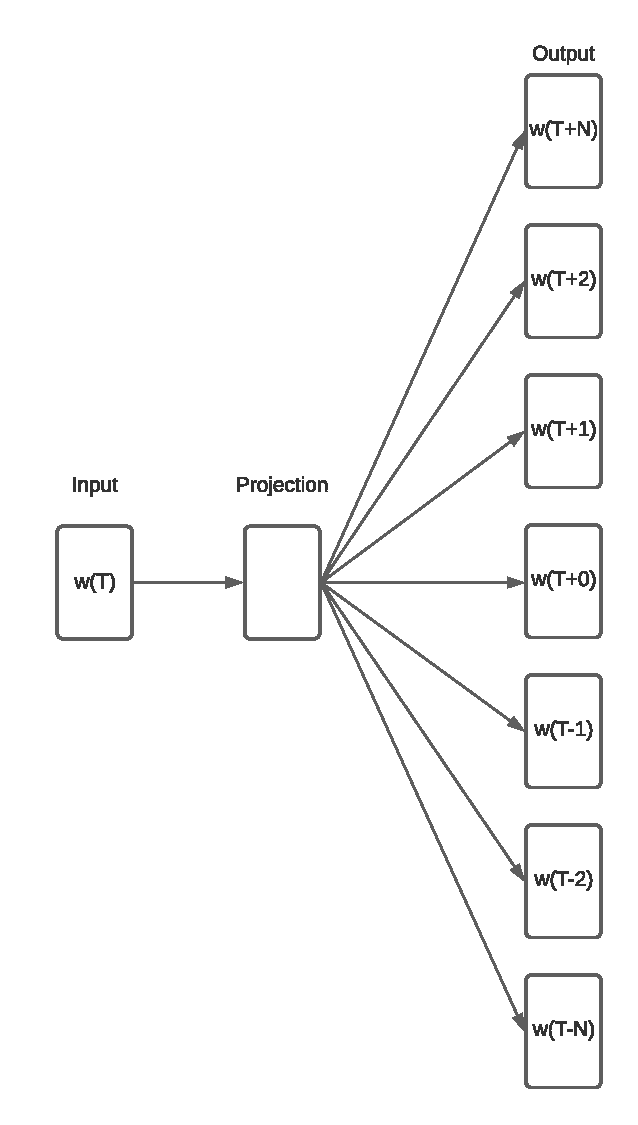
\includegraphics[width=0.49\textwidth]{figures/chapter-5/SkipGramModel.pdf}
    \caption[SkipGramModel]{Input flow of Skip-Gram model.
    \label{fig:SkipGramModel}}
\end{figure}

The skip-gram model can be seen as the inverse of the bag-of-words model as it attempts to vectorize neighboring words first to identify corpus context, whereas, bag-of-words takes each lexeme first, produces a vector sum and then categorises each word.